\documentclass[12pt]{article}
\usepackage[english]{babel}
\usepackage{graphicx}
\usepackage{tabularx}
\usepackage[backend=bibtex, natbib=true]{biblatex}
\usepackage{listings}

\bibliography{bibliography}
%opening
%Here you can enter your names and titleof your report
\title{HIS SSNS - Bi-Weekly Report 3}
\author{
	 Raul Bertone
\and Elis Harruni
\and Muyassar Kokhkharova
\and Saidar Ramazanov
\and Xhoni Robo
}

\begin{document}

\maketitle

%The abstract is used to give a short overview of your report, article, ...
\begin{abstract}
 This report covers the progress made by the group on their project during the time period 31st of May to the 14th of June 2018. Individual and total group effort is at the end of this report.
\end{abstract}

\section{Problems so far}
At the beginning of this two week, the team found itself blocked because we had not found  a way to connect two Sensortags at the same time to either the Launchpad or a PC.\\\\
In the hope of keeping the code we had already written (all Java), and so not waste several weeks of efforts, I concentrated on finding solutions that did not require a change of platform. In particular a switch to Android and/or Python would have represented a major set-back for the team progress: in consideration of the development experience and skill set of the team members, starting on a new development effort with such technologies, would have put us in a worse position than the one we were in at the beginning of the project.\\\\
In consideration of the very little time left to deliver the project, any solution found would have to be very simple to use, ideally an API specifically designed for Bluetooth, or even better a Sensortag project that could be adapted to our use case.\\

\subsection{TinyB}
I found a promising project by Intel called TinyB. This project aims at providing a simple Blutooth API for IOT devices, and it also came with an example specifically using a Sensortag.\\\\
The host part of the Bluetooth stack is implemented in C++, while the API is available in C++ and Java. Since we wanted to use Java, the build and deployment process turned out to be less than straightforward in that it involved using make, a tool tailored for use with C/C++, for an hybrid C++-Java project.\\
Moreover, I had no experience interfacing Java code with other languages, a process that requires the use of the Java Native Interface (JNI).\\
After overcoming all these hurdles, I was presented with a very simple and API and, within minutes, I was able to connect and operate a single Sensortag. Unfortunately there was no build-in way to connect at the same time to more than one Bluetooth server device. From the experience of other users online, I gathered that it is indeed possible, although complex, unreliable and undocumented. In particular everybody seemed to experience constant disconnections when more than one device was connected.\\
At this point I decided to resume my search, in the hope of finding a simpler solution.


\subsection{Kura}
The Eclipse project called “Kura”, a framework for the server side of IOT applications, seemed a good candidate. It contains a Bluetooth LE API which is actually internally based on TinyB. The advantage here is twofold: all the development happens in Java, with the JNI well hidden under several abstraction layers; a Sensortag example is available with a comprehensive API, much more powerful than TinyB on its own. Also there is the hope that multi-device connection would be handled automatically by the framework.\\\\
In general, if we were not so low on time, I wouldn’t have considered Kura as a solution because, while specifically dedicated to IOT development, it is extremely heavyweight. Kura is an OSGI application and requires therefore an OSGI container to be run (for example Eclipse Equinox). This implies the use of pure Linux has the OS (Android in not compatible). This does not fit our scenario as it would require a powerful, and probably non-battery powered device as a Bluetooth base station (at best a Raspberry Pi or similar).\\\\
The next step would be to start working on the available Sensortag example and, again, see if it is possible and easy to connect more than one device.\\

\section{Desktop Application Development}\cite{vendor}\cite{devguide}\cite{userguide}
\textit{This is the report for 4 week since Elis could not report the previous time.}
First a recap of what I was doing I am working all the time with establishing BLE  connection and creating a network to read the required data from the sensors.\\
I started directly with multi\_role project that was suggested to me I could connect tow Slaves to the lunchpad (Master) but to discover Characteristics and read/write I could not do. That happened because the Write/read function of multi role project was not implemented. Considering to implement that function and solve the problem I decided not to do it because of my restricted knowledge on C and C++ from this decision starts the work of this 4 weeks.\\\\
First 2 weeks using host\_test application with lunchpad again as a master I created a network for 1 sensor as a slave reading data and saving them in queue to print on console after that just to see the messages.\\
The implementation was done by the help of Java library to read and write to a serial COM port called jssc.jar.\\\\\\\\\\\\\\\\\\\\
\begin{figure}[h]
	\centering
	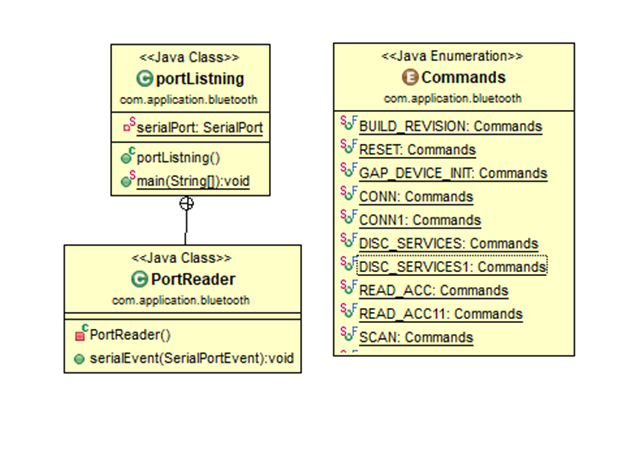
\includegraphics[scale=0.60]{images/UML1.png}
	\caption{UML diagram for the first prototype of Network system in JAVA}
	\label{img:UML1}
\end{figure}
\\First I needed only this three classes portListning PortReader that is a private inner class of port listning and an Enumeration for some commands that I need to send to lunchpad.\\
In the port listning Class the main method search for available COM ports and print them after that it ask you what port want to connect and open. After that activating a SerialPortEvent to the opened port will notify this thread every time that an event is happening to the port write/read.
On the PortReader Class that implements SerialPortEvent Interface implementing the required method serialEvent I only catch read events so when the lunchpad is sendig me data and I just print the hexadecimal Sring in console to check the data.\\
The time consuming part was Creating the so called Commands I started to build commands using TI BLE Vendor Specific HCI Reference Guide BLE5 Version 1.0.0.\\
Creating commands like that was taking a lot of time and I figured out another method sniffing the port with a port sniffer application while I used BLE device monitor for getting data.
Then o got all the writing commands with the help HCI Reference Guide I could translate all messages so I Go only the commands that I need to read from Accelerator. Here I was trying to get data only from Accelerator then later will think for Gyroscope.\\
A the end I could get data for my Application but I need to translate those data and to parse in the way I get a use of them.\\\\
This 2 week I continue on building the NS (Network System) part of SSNS.\\
\begin{figure}[h]
	\centering
	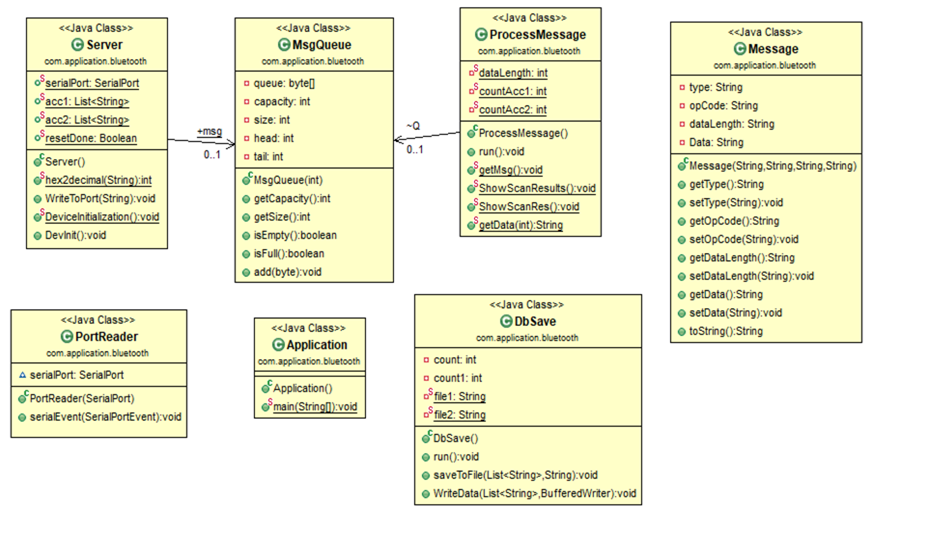
\includegraphics[scale=0.50]{images/UML2.png}
	\caption{New current Application UML diagram.}
	\label{img:UML2}
\end{figure}
\\This is the auto generated UML diagram from an Eclipse plugin that's why there are some relations missing without a detailed explanation this UML is not understandable because of missing elements.
Also here the Commands Enumeration is missing because is very big for the figure.\\
Here we have now 7 classes this is developed from the first Application in previous weeks with 3 classes PortReader is the same but instead of a private inner class now I use Aggregation and Inheritance to implement the same thing. “portListning” was not named good for Java convention by mistake and with the new ideas I got a new name for it that is Server and the main() method now is in a new class Called Application that is somehow the user interface for now(Consloe view).
Now I don’t print the message on the Console when I get an event but insert the byte array to a Byte Queue I implemented and to process the Messages and to parse and translate the messages I use a new thread that gets the data from Queue so I get lower chances to interrupt or to put the main Thread  in a lot of work and risk losing data.\\
I have defined a structure of the every message with the help of TI BLE Vendor Specific HCI Reference Guide BLE5 Version 1.0.0.\\
DbSave class is just a class to save Accelerator data in 2 different files for different sensors.
So with this Structure I can connect 2 sensortags and get data from them in the same time.
Apart for the successful work I was working on developing a python script to read the data from sensor and also with android code from TI but I then gave another try to this before finding a solution on one of those 2.\\


\section{Implementation of Math Model}
On previous weeks was implemented additional functional of Gyroscope method of Fall Detection. As it was mentioned on the last report, the logic of work is:\\\\
First, application should store data from sensors for Gyroscope like for the accelerometer part in parallel mode. Secondly, main mathematical part (accelerometer) should detect a fall. If it happens, the main part should trigger method of Gyroscope class and gives time stamps of the beginning and ending of the fall. Then, Gyroscope part is going to the previous measurements, when falling is started and accelerometer has approximately -1 g on OZ axis. Between these two timestamps, application started to measure angle of the fall on two axis. If composition angle of two axis is equal to:
$$90 \pm 35 \pm 180*n, where n \in Z,$$
then it is mean that patient is laying and Gyroscope class proofs the fall.\\
First problem was to state the timeframe when the fall was. In that point, algorithm looking for the last measurements of \textbf{-1 g} on OZ axis and states it as beginning of fall. Then the end of fall is stated by time when the impact was proceed. By this, we can state the timeframe of the fall for the Gyroscope algorithm.  However, if the measurement of OZ axis is 0 g it means that the user was laying before the fall.\\\\
One of the main problem during the implementation was that the program could not change array of measurements during the computations. That is why there was implemented footprint of the measurements. It brings some disadvantages, as the program should store a lot of information for computations. Nevertheless, it is one solution, which can be done in case to do not lose important measurements from SensorTag.\\\\
Finally, the architecture of the Maths logic now contains three classes:\\
\begin{itemize}
	\item Mathematics – contains main thread of computations, creating stamp of Gyro and Accelerometer objects inside the thread, and contains main static variables like impact power, laying acceleration;
	\item Gyro – contains measurements from sensor, functions off adding new measurements, thread of Gyro computations;
	\item Accelerometer - contains measurements from sensor, functions off adding new measurements, can trigger Gyro method to start its thread.
\end{itemize}

\section{Research and analysis of the Multi\_Role Application}
Due to the constraint as a result of the short amount of time until the end of the project, choosing the best approach is the difference between a successful application and the failure of the project. That is why, while exploring the possibility of using a Java application to connect to the SensorTag, still through the use of the LaunchPad, it would be necessary to continue the research on the Multi\_Role application, as well as understanding how to change the code in order to be able to adapt it to our current needs. Since the documentation on the Multi Role application on the internet is lacking, the best approach would instead be to look at the code and try to understand how it works. To help, we are trying to compare the Multi\_Role application to the Host\_Test application.\\

\subsection{Multi\_Role issues that prevent implementation}
Firstly, the Multi\_Role application is, as mentioned previously, hardly documented. This made it a challenge at first to understand how the application works. After setting up the environment using PuTTY, we were able to use the application. After running the application, everything seemed to work except for the GATT Read/Write operation. In order to track the execution process, we used the debugger feature on Code Composer Studio to track the path of the code, with the hope that it would eventually lead to the function, or at least the file, that handled the Read/Write operation. However, because the application requires input from the LaunchPad buttons in order to execute its functions, the debugger would stop right after the BIOS was initialized, and even though the code would run, no input would be recognized. The alternative approach meant looking at the code itself, and tracking the definition of the methods to get to the right place. Doing so eventually led to the answer that contained the Read/Write function, which consisted of basically an IF statement, that counted the times the operation was successful. Therefore, the main problem became being able to implement a working Read/Write operation.\\

\subsection{Comparing Multi\_Role to Host\_Test}
Due to the constraint as a result of the short amount of time until the end of the project, choosing the best approach is the difference between a successful application and the failure of the project. That is why, while exploring the possibility of using a Java application to connect to the SensorTag, still through the use of the LaunchPad, it would be necessary to continue the research on the Multi\_Role application, as well as understanding how to change the code in order to be able to adapt it to our current needs. Since the documentation on the Multi Role application on the internet is lacking, the best approach would instead be to look at the code and try to understand how it works. To help, we are trying to compare the Multi\_Role application to the Host\_Test application.\\\\
Unlike the Multi\_Role, the Host\_Test application has a higher amount of documentation available. However, the amount is almost infinitely bigger, and finding the small piece of information required to make the implementation of the application is just as difficult as it was for the Multi\_Role. So far, a quick skim of the main documentation given by TI gave us a basic understanding of how the Host\_Test works. However, little of help was given regarding the Read/Write in particular, at least as far as the implementation of it is concerned. More progress will be done until we have a final solution.\\

\section{Effort Hours}
\begin{itemize}
	\item \textbf{Raul Bertone:} 11h
	\item \textbf{Elis Harruni:} 20h
	\item \textbf{Muyassar Kokhkharova:} 13h
	\item \textbf{Saidar Ramazanov:} 15h
	\item \textbf{Xhoni Robo:} 16h\\\\
\end{itemize}

Total Effort: 75h
%----------------------------------------------------------------------------
% Bibliography
%----------------------------------------------------------------------------	
\printbibliography
\end{document}
%----------------------------------------------------------------------------
